%!TEX root = ../thesis.tex
%*******************************************************************************
%*********************************** First Chapter *****************************
%*******************************************************************************
\chapter{Cellular identity in the genomics era}  %Title of the First Chapter
\label{chap:intro}

\ifpdf
    \graphicspath{{Chapter1/Figs/Raster/}{Chapter1/Figs/PDF/}{Chapter1/Figs/}}
\else
    \graphicspath{{Chapter1/Figs/Vector/}{Chapter1/Figs/}}
\fi

Cell biologists have attempted, from the inception of the discipline, to categorize the extensive variability of cells that are found in Nature. This endeavour is hampered by the intrinsic complexity of cells, which associated to their small size and sensitivity to the surrounding environment, makes cellular phenotypes hard to probe in an integrated and comprehensive way. The last decade however has seen extraordinary improvements in the detail to which molecules can be assayed in individual cells. Single-cell RNA-sequencing (scRNA-seq) has for the first time provided an unbiased, transcriptome-wide census of RNA molecules for one cell at a time. By acquiring the transcriptome of large numbers of cells, we can group them by their gene expression programmes - a proxy for their function - and thus define their cell identity. The definition of this cell type identity from the massive amounts of transcriptome data produced in recent years has required the continuous adoption of new computational and analytical methodologies.

This chapter provides an introduction to the definition of cell types. It will show how more recently developed experimental and computational approaches are shaping our understanding of how cells are categorized.


\nomenclature[z-scRNA-seq]{scRNA-seq}{Single-cell RNA sequencing}
\nomenclature[z-RNA]{RNA}{Ribonucleic acid}

%*************************** %First Section  *******************************
\section{Cell type discovery and definition} %Section - 1.1 
\label{section1.1}

%% this paragraph introduces cell biology
The term "cell" was coined by Robert Hooke in the 17th century to describe the empty cell walls he observed in cork samples through his microscope~\citep{hooke_micrographia:_1667}. This observation was complemented some years later, when Antonie van Leeuwenhoek first observed live unicellular organisms and other cells with a microscope composed of more powerful lenses~\citep{mazzarello_unifying_1999}. Research and observations in the following 200 years led to the formulation of cell theory. Its first tenet was introduced by Schleiden and Schwann, and states that all living structures are composed of cells or their byproducts~\citep{schwann_microscopical_1847}. The theory was later complemented by Robert Remak, Rudolf Virchow, and Albert Kölliker to include the postulate that all cells are derived from other cells (in the latin formulation popularized by Virchow, \textit{omnis cellula e cellula}).

%% this paragraph introduces how cellular diversity was classically studied with microscopy
These early studies looked at a variety of sources to unveil different types of cells. Leeuwenhoek reported observations from blood, brain, muscle and semen~\citep{leeuwenhoeck_m_microscopical_1674,leeuwenhoek_antoni_van_observationes_1677}. Subsequent developments of microscopy techniques led to improved imaging of a variety of tissues and the cells that compose them. For the first centuries of cell biology, microscopy was the method of choice to identify cell types. While this was mostly due to the relatively reduced knowledge of cellular biochemistry, it was immediately apparent that morphology was intrinsically tied to cellular function. The most illustrative example of this is the neuron, whose unique structure was only unravelled after subsequent improvements in tissue preparation and staining, as well as increases in resolution and development of electron microscopy~\citep{mazzarello_unifying_1999}. Microscopy was also important in understanding where cell types come from by mapping their developmental origin. The three germ layers - endoderm, mesoderm, ectoderm - were identified in the 19th century, and was postulated that each of them would give rise to different sets of tissues~\citep{collins_terminology_1995}. Developmental studies have since had a central role in defining cell lineages, and thus how cell types are related. Advances in microscopy were also crucial to the identification of organelles. While larger structures, like nuclei, are still identifiable with simpler microscopes~\citep{brown_organs_1866}, others required improved resolution and staining or preparation to be identified~\citep{golgi_structure_1989}. Other advancements in microscopy like live-cell imaging or super resolution microscopy are constantly perfected to expand the boundaries of cellular functional characterization.

%% this paragraph introduces how molecular phenotyping started being used to define cell identity
Advances in biochemistry and molecular biology revealed that most organic molecules that compose cells are directly responsible for their function. Proteins are responsible for most cellular functions, being involved in enzymatic reactions, signalling and regulatory pathways or structural components. They became a prime target for cellular phenotyping with the development of immunostaining~\citep{coons_immunological_1941}, whereby an antibody that specifically targets a certain protein is usually tagged with a fluorophore. Immunostaining can identify protein expression in tissue slices, and the use of different fluorophores allows for the imaging of cells expressing multiple proteins. The usefulness of immunostaining became especially apparent when it was combined with high-throughput microfluidics methods and used for fluorescence-activated cell sorting (FACS)~\citep{bonner_fluorescence_1972}. This introduced the first high-throughput studies on molecular phenotyping of cells, and sorting allowed cell function to be probed in parallel~\citep{julius_demonstration_1972}. More recently, mass cytometry has allowed for a further expansion of the repertoire of proteins assayed~\citep{bandura_mass_2009,di_palma_unraveling_2015}. This technique, while destructive, has also been combined with tissue imaging, adding a spatial component to the cell populations examined~\citep{chang_imaging_2017}.

%% this last paragraph lists the gaps that had to be filled by genomics for cell biology
The identification and classification of cell types is dependent on their function. Function is deeply related to cellular morphology~\citep{prasad_cell_2019}, and both are ultimately a consequence of the molecular pathways shaping them. Additionally, even though recent advances permit high throughput cell sorting through imaging~\citep{nitta_intelligent_2018}, the limited resolution hinders the identification of finer details of cell and organelle shape, which are frequently more informative of cellular activity. Cell sorting with fluorescent antibodies and mass cytometry can reveal more details on the molecules underlying cellular behaviour, but they are targeted approaches that depend on prior knowledge of the effector molecules. The more recent attempts at defining cell identity have therefore relied on the unbiased, high-throughput character of single-cell RNA-sequencing methods.


\nomenclature[z-FACS]{FACS}{Fluorescence-Activated Cell Sorting}

%********************************** %Second Section  *************************************
\section{Defining cell types using scRNA-seq} %Section - 1.2
\label{section1.2}

%% history of the growth of scRNA-seq
Methods to sequence the transcriptome of individual cells started to be developed shortly after the advent of RNA-seq~\citep{mortazavi_mapping_2008,tang_mrna-seq_2009}. This early development was pushed not by a need to define the molecular makeup of the unit of life, but rather to allow transcriptomic studies to be performed in low-input samples. Nonetheless, this seminal work still sparked the improvements that occurred in the decade that followed~\citep{svensson_exponential_2018} (Figure~\ref{fig:chap1_fig1}).

\begin{figure}[ht!]
    \centering    
    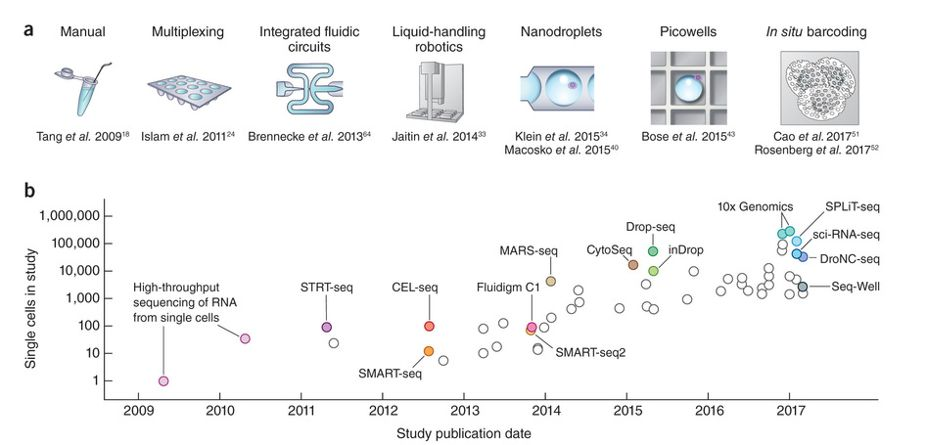
\includegraphics[width=1.0\textwidth]{Chapter1/Figs/chap1_fig1.jpg} % change word in curlies to change figure
    \caption[Timeline of scRNA-seq technology development]{\textbf{Timeline of scRNA-seq technology development}\newline\textbf{(A)} Key technologies that have allowed jumps in experimental scale. A jump to \texttildelow100 cells was enabled by sample multiplexing, and then a jump to \texttildelow1,000 cells was achieved by large-scale studies using integrated fluidic circuits, followed by a jump to several thousands of cells with liquid-handling robotics. Further orders-of-magnitude increases bringing the number of cells assayed into the tens of thousands were enabled by random capture technologies using nanodroplets and picowell technologies. Recent studies have used in situ barcoding to inexpensively reach the next order of magnitude of hundreds of thousands of cells. \textbf{(B)} Cell numbers reported in representative publications by publication date. Key technologies are indicated. \textit{Original figure published in~\citep{svensson_exponential_2018}.}}
    \label{fig:chap1_fig1}
\end{figure}

Initial developments focused on increasing sensitivity, since the original scRNA-seq protocol was performed on cells from very early developmental stages, which are larger and contain more RNA than most differentiated cell types. Different methodologies quantified gene expression by sequencing distinct transcript segments (either the 5' or the 3' end, or the full transctipt)~\citep{islam_characterization_2011,hashimshony_cel-seq:_2012,ramskold_full-length_2012,picelli_full-length_2014}. The idea of multiplexed scRNA-seq also started gaining traction with the use of multi-well plates or molecular barcodes for cells. The company Fluidigm eventually introduced the first commercially available microfluidics chips (called the "Fluidigm C1 system") for miniaturized cell isolation, RNA extraction and reverse transcription~\citep{brennecke_accounting_2013}. It is from this point that increased cell capture becomes the major technological driver (and has gained even great importance as discussed in Section \ref{section1.3}). The major contributors to this have been nanodroplet-based technologies, that have put the number of profiled cells per dataset in the range of 10.000 to 100.000~\citep{macosko_highly_2015,klein_droplet_2015}. The importance of this increase in throughput has been demonstrated by Shekar and colleagues~\citep{shekhar_comprehensive_2016}, where they demonstrate that a Drop-seq dataset of approximately 25.000 cells sequenced at low depth could identify more \textit{bona fide} cell types and subtypes than a smaller, more deeply sequenced Smart-seq2 dataset. Currently, most single-cell RNA-seq datasets use droplet-based technologies, chiefly the protocols designed for the Chromium instrument by 10x Genomics~\citep{zheng_massively_2017}, which have a higher sensitivity to detect different transcripts. Other more recent methods have followed the trend of increase in cell throughput by using multiplexed barcoding, which allows for different samples to be combined and reducing sample processing costs, reaching 10\textsuperscript{5}-10\textsuperscript{6} cells for less than \$0.01 per cell ~\citep{rosenberg_single-cell_2018,cao_single-cell_2019}. A list of the most up-to-date scRNA-seq methods can be found in Table~\ref{table:tab_1_1}.

% table: Method; Ref
\begin{table}[ht!] % p for putting it in the next page available
\footnotesize
\caption[Current methods for single-cell RNA-seq]{Current methods for single-cell RNA-sequencing}
\centering
\label{table:tab_1_1}
\begin{tabular}{l|l|c}
\toprule
~\textbf{Method Name} & ~\textbf{Reference}  \\
\midrule
Fluidigm C1 & ~\citep{brennecke_accounting_2013}  \\

Smart-seq2 & ~\citep{picelli_full-length_2014}  \\

Drop-seq & ~\citep{macosko_highly_2015}  \\

inDrop & ~\citep{klein_droplet_2015}  \\

CEL-seq2 & ~\citep{hashimshony_cel-seq2:_2016}  \\

Chromium & ~\citep{zheng_massively_2017}  \\

ICELL8 & ~\citep{goldstein_massively_2017}  \\

Quartz-seq2 & ~\citep{sasagawa_quartz-seq2:_2018}  \\

mcSCRB-seq & ~\citep{bagnoli_sensitive_2018}  \\

SPLiT-seq & ~\citep{rosenberg_single-cell_2018}  \\

MARS-seq2 & ~\citep{keren-shaul_mars-seq2.0:_2019}  \\

sciRNA-seq3 & ~\citep{cao_single-cell_2019}  \\

Seq-Well S\textsuperscript{3} & ~\citep{hughes_highly_2019}  \\

\bottomrule
\end{tabular}
\end{table}

%% methods to discover cell types (with some examples)
The exponential developments in single-cell sequencing technologies were accompanied by essential computational developments to analyse the resulting data. From a cell type discovery perspective, the key methods are clustering and pseudotime analysis~\citep{rostom_computational_2017}, which assign to cells a discrete or a continuous label, respectively. These are of course dependent of the upstream processing steps of normalisation, feature selection and dimensionality reduction, as well as often used batch correction methods~\citep{luecken_current_2019}. Most of these analysis steps are available in accessible software toolkits~\citep{mccarthy_scater:_2017,butler_integrating_2018,wolf_scanpy:_2018}.

With clustering, the goal is to identify discrete cell populations. The most widely used methods for clustering are the louvain and leiden community detection algorithms~\citep{blondel_fast_2008,traag_louvain_2019}. These populations are commonly considered an approximation of the cell types present in a sample of dataset, often justified by examining the presence of known markers for known cell types across clusters. Further application of differential expression methods (extensively benchmarked in~\citep{soneson_bias_2018}) between clusters can identify other potentially novel genes that are, within that context, unique to that population. This can be used to characterise newly discovered populations~\citep{villani_single-cell_2017,montoro_revised_2018,shekhar_comprehensive_2016} and to identify new markers that can be used to isolate or understand known cell types~\citep{shulse_high-throughput_2019,vento-tormo_single-cell_2018,bjorklund_heterogeneity_2016}.

Pseudotime analysis consists on describing a set of cells from a continuous perspective. The name derives from the original application to obtain a dimensionless temporal trajectory from time course scRNA-seq data~\citep{trapnell_dynamics_2014}. There are several methods to perform this analysis (exhaustively reviewed in ~\citep{saelens_comparison_2019}), all with the goal of defining a latent variable from the data along which a biological process, reflected in gene expression, is changing. Pseudotime is especially useful to study response to stimuli ~\citep{trapnell_dynamics_2014,lonnberg_single-cell_2017} and developmental trajectories ~\citep{cao_single-cell_2019,watcham_new_2019}, but has also been used to model changes to cellular spatial distribution ~\citep{scialdone_resolving_2016}. These methods can differ in the way they model biological trajectories, with some explicitly allowing for branched trajectories. This is of special importance in development, where the goal is usually understanding which daughter cell types share  progenitors. The direction of differentiation is usually just assumed according to previous knowledge and of the experimental conditions. This is not completely possible in all situations, yet can be inferred from expression data. By considering RNA kinetics, and using the quantification of spliced/unspliced reads, the current and future (i.e. still circumscribed to the nucleus) transcriptomic states can be untangled as a "velocity" vector~\citep{manno_rna_2018}. In differentiation trajectories, cell types are therefore usually defined as the endpoints, with the cells in between forming more transient cell states, along which gene expression is dynamically adjusting to the final cellular identity. It should be noted that this "cell type vs cell state" nomenclature is context-dependent, and there is no absolute agreement on how cell types should be formally and empirically defined~\citep{noauthor_what_2017}. 

%% advantages and disadvantages of using scRNA-seq, and how it can be complemented
Globally, the increasing adoption of scRNA-seq is due to its multi-gene and unbiased profile. It allowed for the first time the non-directed profiling of molecules driving heterogeneity in cellular populations. Nonetheless, its use for defining cell identity still has some drawbacks. Even though the cost of high-throughput sequencing keeps dropping, single-cell RNA-seq still requires costly protocols, especially at the scale that it is currently performed for cell type discovery. This however can be mitigated by more targeted approaches, aimed at characterizing specific subsets of already known cell types isolated by their broad markers. scRNA-seq is also prone to batch effects, which can become more pronounced when comparing or integrating data generated by different protocols. This has been a very active topic of research, and several batch alignment and correction methods can now account for these integration of different protocols~\citep{butler_integrating_2018,haghverdi_batch_2018,park_fast_2018,stuart_comprehensive_2019}. From the protocol side, sample barcoding for multiplexed processing also greatly reduces batch issues~\citep{stoeckius_cell_2018,shin_multiplexed_2019}.

One last concern, although perhaps the largest, is the fact that profiling a tissue or a cell type with scRNA-seq does not inherently give any functional information about the cells. Cellular function has been from the beginning the major point to categorize cells. RNA, despite being easily correlated with protein presence, is not in most cases the effector molecule in a biological process. Additionally, most single-cell methodologies destroy the cell without imaging it, making the link between molecular makeup and morphology harder to obtain. While this is an ongoing research topic, profiling cells through the use of multi-omics technologies can help obtain a deeper mechanistic characterization. Information on open chromatin regions~\citep{buenrostro_single-cell_2015}, histone modifications~\citep{kaya-okur_cut&tag_2019} or surface proteins~\citep{stoeckius_simultaneous_2017} have the potential to be combined, directly or indirectly, with single-cell RNA-seq~\citep{clark_scnmt-seq_2018}. This can provide information on how these molecular layers interplay and learn about the intrinsic regulatory processes of gene expression~\citep{gorin_rna_2019,qiu_mapping_2019}. CRISPR screens with single-cell expression readout can also reveal more about cellular function~\citep{dixit_perturb-seq:_2016,datlinger_pooled_2017}. Lastly, developments in spatial transcriptomics hold the promise of providing spatial context to cellular transcriptomes profiled individually, providing information on the tissue context for cell identity determination~\citep{vickovic_high-density_2019,rodriques_slide-seq:_2019}. Overall, while the discussion about where to draw the line between cell types still lasts, technological developments provide us with ever increasing information to approach a decisive and informative definition.



%********************************** % Third Section  *************************************
\section{Methods for cell type classification}  %Section - 1.3 
\label{section1.3}

%% using scRNA-seq to build cellular atlases
Single-cell RNA-seq was initially developed to obtain the whole transcriptome from samples with very low starting material~\citep{tang_mrna-seq_2009}. Nonetheless, the notion of using it to define cell types through their transcriptome was very early on envisioned. In 2011, Islam and colleagues end the discussion on their newly developed scRNA-seq method (STRT-seq) by stating "We envisage the future use of very large-scale single-cell transcriptional profiling to build a detailed map of naturally occurring cell types, which would give unprecedented access to the genetic machinery active in each type of cell at each stage of development."~\citep{islam_characterization_2011}. The exponential increase in the number of cells profiled per experiment eventually made this prediction come true. A large amount of single-cell projects have used the technology to profile cells captured from various tissues, in steady-state or disease conditions. Yet the most direct example of how this quote reflects the evolution of the field is the Human Cell Atlas (HCA)~\citep{regev_human_2017}. This consortium has been established as a forum for scientists around the world to share their expertise on genomics, bioinformatics, and tissue biology, and coordinate the high-throughput profiling of cellular heterogeneity in the human body. The HCA has groups focusing not just on individual organs, but also on development~\citep{behjati_mapping_2018,taylor_pediatric_2019} and disease. 

In parallel, there have been increased efforts to obtain similar references for other species, in particular animal models~\citep{fincher_cell_2018,cao_comprehensive_2017}. The data collected for these species tends to have a greater cell coverage since the tissue samples can be more readily available. Furthermore, these atlases are by no means less important or useful than the human reference. The cell atlases produced for mouse~\citep{han_mapping_2018,noauthor_single-cell_2018} were of especial relevance, since they constitute the first broad, multi-organ cellular census of a mammalian organism, and one for which a large portion of biomedical science has relied on. The accessibility of human tissues for profiling and ~\textit{in vitro} testing will be crucial in the near future. Nonetheless, having a mouse reference that can be related to human can not only teach us about the evolutionary principles that shape cell type evolution through gene expression, but also serve as a bridge to transpose mouse-based biomedical discoveries into a human context.

% table: Title; Description; Ref
\begin{table}[p] % p for putting it in the next page available
\footnotesize
\caption[Methods for automated cell state matching]{Comprehensive list of papers detailing methods for automated cell state matching}
\centering
\label{table:tab_1_2}
\begin{tabular}{l|l|c}
\toprule
~\textbf{Method Name} & ~\textbf{Short Description} & ~\textbf{Reference}  \\
\midrule
scmap & \specialcell[t]{k-nearest-neighbor search\\with cosine distance} & ~\citep{kiselev_scmap:_2018}  \\

matchSCore & Jaccard Index for cluster markers & ~\citep{mereu_matchscore:_2018}\\

ClusterMap & \specialcell[t]{Hierarchical clustering with\\marker gene binary expression} & ~\citep{gao_clustermap:_2018}\\

CaSTLe & XGBoost classification & ~\citep{lieberman_castle_2018}\\

Moana & Linear SVM on (sub)clusters & ~\citep{wagner_moana:_2018}\\

SAVER-X & Autoencoder & ~\citep{wang_transfer_2018}\\

scQuery & Neural network classifier & ~\citep{alavi_web_2018}\\

PopAlign & \specialcell[t]{oNMF, Gaussian Mixture model\\and Jeffrey’s divergence} & ~\citep{chen_dissecting_2018}\\

scGen & VAE and linear classifier & ~\citep{lotfollahi_generative_2018}\\

scVI & VAE and hierarchical Bayesian model & ~\citep{lopez_deep_2018}\\

scPred & SVM in principal component space & ~\citep{alquicira-hernandez_scpred:_2018}\\

SingleCellNet & \specialcell[t]{Random Forest on\\binary marker expression} & ~\citep{tan_singlecellnet:_2018}\\

CellAssign & \specialcell[t]{Multi-variable model with marker genes 
\\and hierarchical Bayesian framework} & ~\citep{zhang_probabilistic_2019}\\

ACTINN & Neural network & ~\citep{ma_automated_2019}\\

scID & \specialcell[t]{Linear Discriminant Analysis\\with marker genes} & ~\citep{boufea_scid:_2019}\\

SingleR & Spearman correlation with training data & ~\citep{aran_reference-based_2019}\\

Garnett & \specialcell[t]{Elastic net multinomial classifier using\\markers from hierarchical cell types} & ~\citep{pliner_supervised_2019}\\

SCINA & bimodal distribution of signature genes, & ~\citep{zhang_scina:_2019}\\

Cell BLAST & \specialcell[t]{Adversarial Autoencoder and\\nearest neighbour search} & ~\citep{cao_cell_2019}\\

scMatch & \specialcell[t]{Correlation with individual sample\\or average of references} & ~\citep{hou_scmatch:_2019}\\

SuperCT & Neural network with binary expression & ~\citep{xie_superct:_2019}\\

CellO & Hierarchical binary classifiers & ~\citep{bernstein_hierarchical_2019}\\

\specialcell[t]{scCoGAPS \&\\projectR} & NMF and projection in that latent space & ~\citep{stein-obrien_decomposing_2019}\\

SciBet & \specialcell[t]{Entropy test and Bayesian comparison\\of multinomial distributions} & ~\citep{li_scibet:_2019}\\

Seurat "Anchors" & \specialcell[t]{CCA, L2-normalisation and\\mutual nearest neighbours} & ~\citep{stuart_comprehensive_2019}\\

LIGER & integrative NMF and joint clustering & ~\citep{welch_single-cell_2019}\\

cellHarmony & \specialcell[t]{Correlation with cluster centroids\\of mean marker gene expression} & ~\citep{depasquale_cellharmony:_2019}\\

CHETA & \specialcell[t]{Correlation with marker genes of\\hierarchical reference} & ~\citep{de_kanter_chetah:_2019}\\

scPopCorn & \specialcell[t]{Co-membership Propensity Graph and\\(joint) k-partition} & ~\citep{wang_subpopulation_2019}\\

p-DCS & Voting based on known marker genes & ~\citep{domanskyi_polled_2019}\\

EnClaSC & Ensemble neural network classifier & ~\citep{chen_enclasc:_2019}\\

scClassify & \specialcell[t]{Ensemble classifier from\\inferred cell type tree} & ~\citep{lin_scclassify:_2019}\\

\bottomrule
\end{tabular}
\end{table}

%% most relevant methods for cell type classification
For a cell atlas to be used as a reference, it needs not only the expression data to be annotated, but also a computational framework that can use it to classify new datasets of interest. Over the last two years, several methods have been developed to handle scRNA-seq data (a comprehensive list can be found in Table~\ref{table:tab_1_2}), which can be added to other general purpose classification methods. These methods vary in complexity, but in general they rely on machine learning approaches to map the reference cell labels to the target dataset. While the most accurate method for this classification is still up for debate (see~\citep{abdelaal_comparison_2019,kohler_deep_2019} in addition to benchmarks in individual method papers), there is agreement about the major challenges for this task. Classification methods should be aware of batch differences, be they caused by use of different scRNA-seq protocols or other technical differences in tissue processing. Different cell isolation and library preparation protocols can have a large impact on the number and type of genes detected~\citep{mereu_benchmarking_2019}.

Many methods also mention the need to build a comprehensive reference, that should be integrated taking the into account the technical variability mentioned above. Training, and especially the prediction phases of the method should also be scalable. Models can take a very long time to train on larger references, and prediction steps that involve extensive manipulation or transformation of the target data can become time consuming with the ever growing size of expression matrices. 

Lastly, some methods try to approach this classification problem from a hierarchical point of view~\citep{wagner_moana:_2018,pliner_supervised_2019,lin_scclassify:_2019}. This is based on the notion that cell types can be organised trees depicting phenotypic relationships. These trees represent not just developmentally-related lineages, but also the increasing specification of cellular function (still mostly correlating with terminal differentiation). This can be of great value in instances like describing cells from the immune system or the brain, where functional diversification leads to more intricate phenotypes (see Section \ref{section1.4}). Notwithstanding, a hierarchical classification can also be seen as a method that reflects the uncertainty in the prediction. Each individual cell ideally conforms to a determined phenotype, which would correspond to a leaf node in an ideal cell hierarchy. Assigning a cell to a parent node rather than a terminal one (or not doing it with a high confidence) can be caused by data sparsity or low coverage, and thus not necessarily reflecting a naturally occurring hierarchy of gene expression-driven cellular phenotypes. Yet this structure is intuitive and informative, and projects like the Cell Ontology have considerable value in creating a controlled vocabulary to name and relate cell types~\citep{bard_ontology_2005}, with some of the methods listed here explicitly conforming to it. The use of a curated and specific nomenclature should thus be incentivized when doing ~\textit{de novo} annotation of scRNA-seq data, and supplying these labels can greatly accelerate the data interpretation and its application in the development of new algorithms.

%% brief discussion on classification (what sort of data? what can we learn from this sort of methods?)
Large collections of data and development of informative references can be of multiple uses. A steady-state cell identity reference can serve as a baseline to which a disease sample can be compared. Having a sufficiently comprehensive reference can do away with the need to generate a new control dataset every time the cellular aspects of a disease are studied through scRNA-seq. Evolutionary biology can also benefit from predictive models for cell identity. Models can be adapted to function across species, which can help trace the evolutionary origins of cell types. Producing interpretable models from integrated data can also be informative in itself. Some models return the importance of genes or gene sets in classifying each cell type, and as such can help uncover novel features of a cell's phenotype. Finally, organised references can also speed up new in-depth studies of specific cell types, as well as studies focusing on other aspects of cell identity (e.g. open chromatin, methylation, proteome, or spatial interactions). It should be noted that the methods discussed so far in this section, while being in their majority developed for scRNA-seq, can also for the most part be adapted to other data modalities like scATAC-seq (for open chromatin) or CITE-seq (combining RNA and surface protein detection). Modelling cell identity with multiple layers can revel more details about the molecules shaping it, how they interact, and their relative importance.


\nomenclature[z-HCA]{HCA}{Human Cell Atlas}
\nomenclature[z-SVM]{SVM}{Support Vector Machine}
\nomenclature[z-NMF]{NMF}{Non-negative Matrix Factorization}
\nomenclature[z-oNMF]{oNMF}{orthogonal Non-negative Matrix Factorization}
\nomenclature[z-VAE]{VAE}{Variational Autoencoder}
\nomenclature[z-scATAC-seq]{scATAC-seq}{single-cell Assay for Transposase-Accessible Chromatin sequencing}
\nomenclature[z-CITE-seq]{CITE-seq}{Cellular Indexing of Transcriptomes and Epitopes by sequencing}

%********************************** % Fourth Section  *************************************
\section{Cell identity in the immune system}  %Section - 1.4 
\label{section1.4}

%% Introduction to the cells in the immune system
%% examples of single-cell (immune dev, cross-tissue het, within tiss het,...)
The immune system is one of the most complex and diverse biological systems across the animal kingdom. The increased evolutionary pressure caused by the need to continuously adapt to the fast evolving pathogens~\citep{barreiro_evolutionary_2010} has resulted in a broad variety of molecular pathways and cells. The variability in the types of cells found in the immune system is directly related to their intrinsic plasticity in gene expression. Immune cells are very responsive to their environment, having to constantly fine-tune expression programmes to react in a prompt and targeted manner. It then comes as no surprise that many cell states have been determined and named in immunology, and it is, perhaps on par with neurobiology, the field where the definition of cell type and cell state clash the most. 

Due to the fact that immune cells are non-adherent cells, immunology benefited immensely from the development of flow cytometry. Immune cells have been deeply characterised by this technology, with antibodies targeting surface receptors as well as cytoplasmic proteins. It then comes as no surprise that the immune system has been an early and major target of single-cell sequencing methods. scRNA-seq has had a role in the fine-grained mapping of gene expression changes in haematopoiesis~\citep{watcham_new_2019}, discovering and reorganising subpopulations~\citep{villani_single-cell_2017}, mapping their heterogeneity across tissues~\citep{miragaia_single-cell_2019,scott_transcription_2018}, studying immune response to pathogens~\citep{lonnberg_single-cell_2017,stubbington_t_2016}, and map communication of immune cells with their tissue of residence~\citep{vento-tormo_single-cell_2018}.

%% Introduction to helper T cell heterogeneity
%% blurring boundaries of cell type/cell state
Immunity can be divided into innate and adaptive. The latter depends on a subset of lymphocytes which are responsible for an immune response that can flexibly adjust to invading pathogens in a non-evolutionary way (i.e. without the need for selection at the level of the individual). The key strength of this system is the use of receptors which recombine and mutate~\citep{krangel_mechanics_2009}, forming a highly diverse repertoire that can eventually be selected to respond to particular invaders. This variability, central to the adaptive immune response, is further complemented by immune memory, that is, the specific repertoire obtained when combating an infection will remain stored in the organism in the form of inactive immune cells, which can be more quickly reactivated should the same threat reappear. This is far more advantageous than having to undergo selection of the receptor repertoire every time the same pathogen is introduced in the system.

\begin{figure}[ht!]
    \centering    
    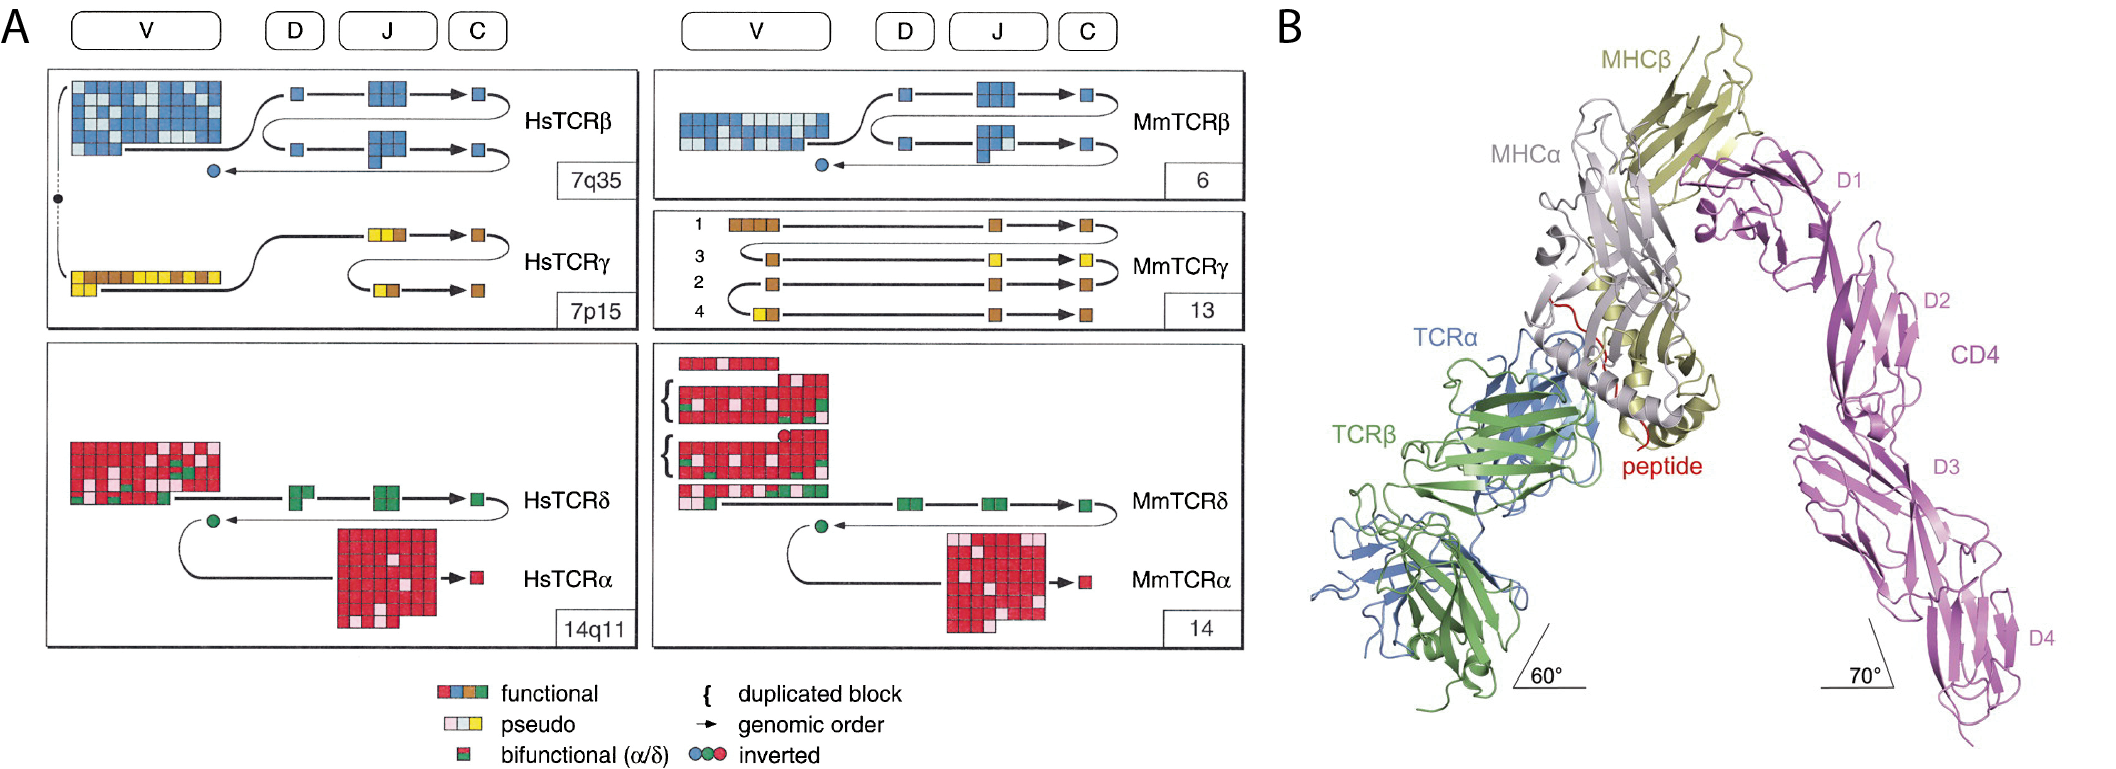
\includegraphics[width=1.0\textwidth]{Chapter1/Figs/chap1_fig2.png} % change word in curlies to change figure
    \caption[Gene and protein structure of TCR]{\textbf{Gene and protein structure of TCR}\newline\textbf{(A)} The genomic organization of the human (left) and mouse (right) TCR genes ${\upalpha}$ (red), ${\upbeta}$ (blue), ${\upgamma}$ (brown), and ${\updelta}$ (green), showing clusters of V, D, J, and C gene segments aligned vertically for clarity. Arrows represent the direction of transcription within each of the TCR genes; squares and circles indicate gene elements in the direct and reverse orientations, respectively. The murine TCR ${\upgamma}$2 gene is inverted relative to the rest of the locus. Dark colors indicate apparently functional gene elements, while lighter shades represent pseudogenes. Curly brackets indicate the duplicated sets of V genes in murine TCR ${\upalpha}$/${\updelta}$ locus. The TCR ${\upbeta}$ and TCR ${\upgamma}$ loci are both on human chromosome 7, on opposite sides of the centromere (schematically represented by the black circle). \textit{Original figure published in~\citep{glusman_comparative_2001}.}\newline\textbf{(B)} Ribbon diagram of the complex oriented as if the TCR MS2-3C8 and CD4 molecules are attached to the T cell at the bottom and the HLA-DR4 MHC class II molecule is attached to an opposing APC at the top. TCR ${\upalpha}$ chain, blue; TCR ${\upbeta}$ chain, green; CD4, pink; MHC ${\upalpha}$ chain, gray; MHC ${\upbeta}$ chain, yellow; MBP peptide, red. \textit{Original figure published in~\citep{yin_crystal_2012}.}}
    \label{fig:chap1_fig2}
\end{figure}

Within adaptive immunity lymphocytes, T cells fill various niches, but are broadly considered to be the orchestrators of immune response~\citep{kumar_human_2018}. T cells are characterised by their expression of the T Cell Receptor (TCR), a dimeric surface protein that can recognise an antigen presented by an Antigen Presenting Cell (APC)~\citep{reinherz_revisiting_2014}. This receptor's capability in recognizing a trove of antigens resides in the original gene's characteristic recombination capabilities. TCR genomic segments contain, in addition to a constant region, many genes - grouped into variable (V), diversity (D) and junction (J) genes - that encode for the variable section of the final protein, which interacts with the presented antigen (Figure~\ref{fig:chap1_fig2}A). These genes are recombined during T cell development in the thymus through the action of RAG enzymes, which target recombination signal sequences to cleave the DNA and join different segments - first D and J (if D is present), then (D)J and V - often with the insertion of additional nucleotides, resulting if further variability. V and J genes are numerous, which results in a very large number of possible V-J combinations, thus ensuring the flexibility for antigen recognition of T cells. This is further augmented by differential combination of TCR chains in the final receptor. The activity of each receptor sub-unit is subject to selective pressures that ensure that it can functionally recognise and respond to foreign antigens, while being unresponsive to self-produced peptides and thus avoid auto-immune responses. In adaptive T cells, these receptors are composed of an ${\upalpha}$ and a ${\upbeta}$ chain. ${\upgamma}$ and ${\updelta}$ chains also exist as a pair, but are less variable which results in a different type of response~\citep{simoes_molecular_2018}.

The TCR is part of a larger membrane surface complex that assists in the recognition of the antigen being presented, as well as the APC presenting them (Figure~\ref{fig:chap1_fig1}B). T lymphocytes can thus be separated into two subsets with a shared developmental origin, bifurcating depending on the type of antigen-presenting Major Histocompatibility Complex (MHC) they can match. Consequently, each with their own APC matching capabilities and is easily identifiable by the expression of a surface protein that participates in this specific interaction. CD8-expressing T cells recognise antigens presented through MHC class I, which exists on the surface of almost all cells. This recognition elicits the maturation of CD8\textsuperscript{+} T cells, preparing them for an anti-cellular response. This subset is accordingly also named cytotoxic, and through the use of perforins and granzymes they destroy cancer cells, as well as cells infected by intracellular pathogens~\citep{halle_mechanisms_2017}.

\begin{figure}[ht!]
    \centering    
    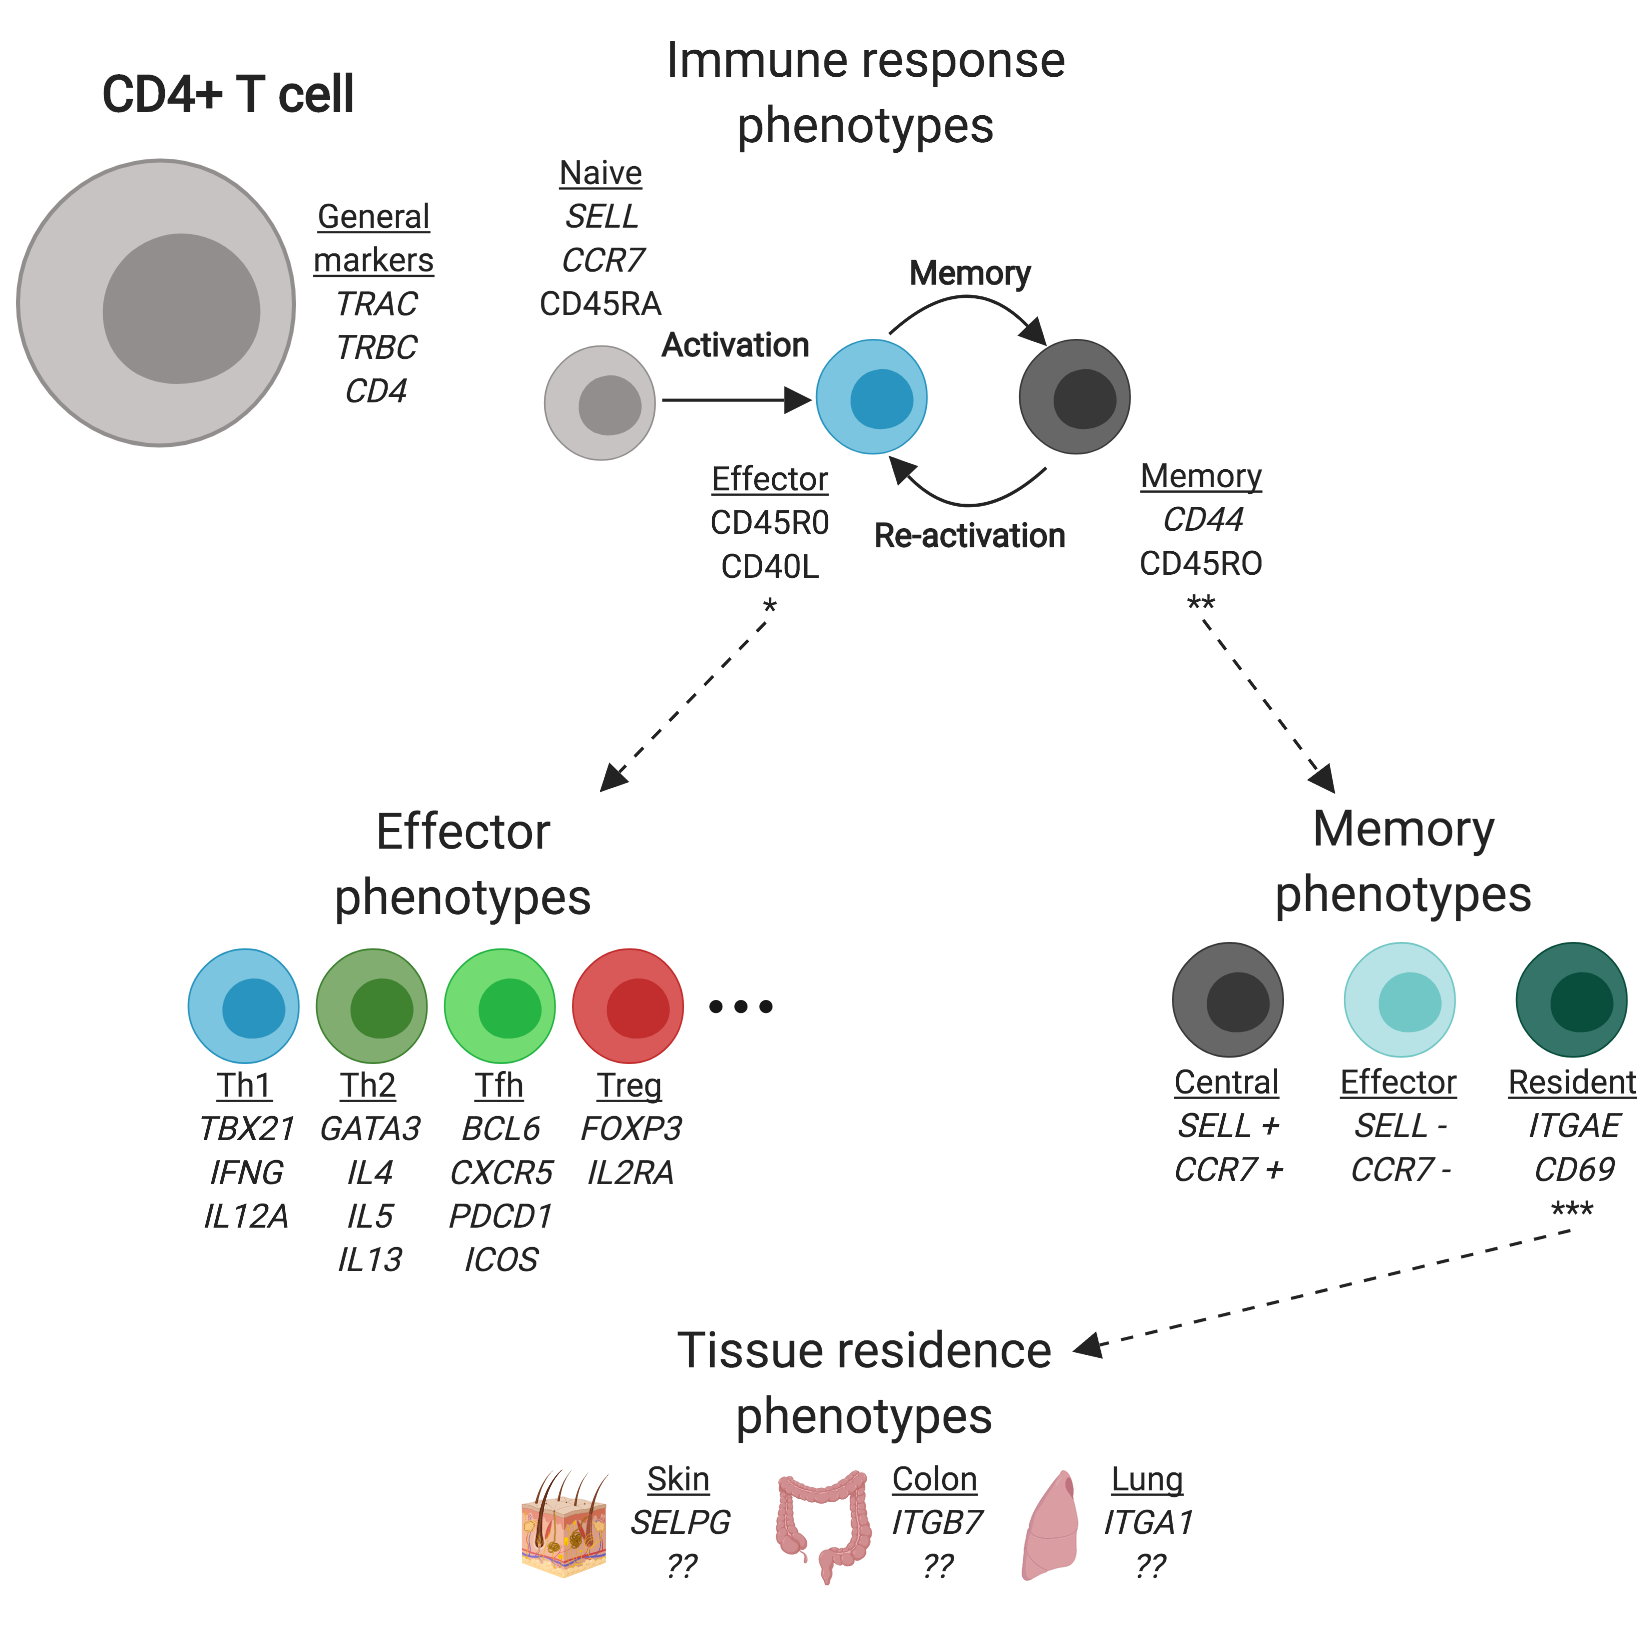
\includegraphics[width=1.0\textwidth]{Chapter1/Figs/chap1_fig3.png} % change word in curlies to change figure
    \caption[T-helper cell heterogeneity and key marker genes]{An overview of known T-helper cell heterogeneity and key marker genes. Beyond their core markers, Th cells can be classified into based on different phenotypes that depend on stage of immune response, the type of effector function, the type of memory cell they form and their tissue of residence (a topic understudied comparatively to the rest). Question marks (??) represent unresolved phenotypes.}
    \label{fig:chap1_fig3}
\end{figure}

CD4\textsuperscript{+} T cells are the other lineage of T cells. Also known as T-helper (Th) cells, these lymphocytes are credited with the organisation of immune response, producing cytokines that serve as triggers or blockers of particular immune reactions~\citep{luckheeram_cd4+t_2012}. Th cells recognise antigens presented by the MHC class II, present only on the membrane of dendritic cells, mononuclear phagocytes, some endothelial cells, thymic epithelial cells (important during T cell selection for functional, non-self-responding TCR), and B cells. This interaction, combined with signalling from the media where the cell is acting, induce an activation programme of the cell that is specific to the external threat being handled. CD4\textsuperscript{+} T cells encompass a large transcriptional plasticity, which results in diverse related phenotypes (Figure~\ref{fig:chap1_fig3}). Th cells have classically been organised into various effector phenotypes on the grounds of their cytokine output~\citep{mosmann_two_1986,schmitt_regulation_2015}, allowing them to coordinate the action of particular cell types, in agreement with the type of immune response at hand. IFN${\upgamma}$ production by Th1 cells has been identified as a key signalling molecule to combat intracellular parasites through the stimulation of macrophages, as well as class switch recombination of B cells to an IgG isotype. In turn, Th2 cells use IL-4 and IL-13 to stimulate basophils and mast cells to release granules against helminth invaders, and Th17 cells coordinate neutrophil recruitment by epithelial cells through IL-17A and IL-17F~\citep{weaver_th17_2013}. While diverse in function, these effector phenotypes are not the sole drivers of variability between Th cells, rather they exist in parallel with other expression programmes. 

Upon finishing responding to an infection, T cells can go into a lowly replicative memory state in which they will save the TCR that drove the specialized response. The various memory states relate to the level of activation of the cell, but also to its tissue of residence. Cells expressing the chemokine receptor CCR7 are in a more naive, non-stimulated state, and also target lymphoid tissues like lymph nodes or the spleen, where most of antigen presenting to CD4\textsuperscript{+} T cells takes place. In addition, tissue-homing and residency phenotypes exist, all of them characterised by the involvement of one or more chemokine receptors or adhesion molecules like integrins. Nonetheless, tissue-specificity in T-helper cells, and even more broadly in immune cells, is still generally understudied. Recent developments using single-cell high throughout methods have tackled this questions~\citep{wong_high-dimensional_2016,scott_transcription_2018}, and it is expected that future efforts will rely on the accumulation of data to extract these patterns from cross-tissue samples.

%% regulation and plasticity of T cell identity (mention Treg functions, mention homeostatic functions)
Among the phenotypic variability of T-helper cells we can find the particular subset termed T-regulatory (Treg) cells. They are different from most Th cell subtypes in that, rather than boosting immune response, they are responsible for dampening it~\citep{sakaguchi_immunologic_1995}. This regulatory role in the immune system is of dire importance. Leaving the immune response unchecked can lead to destructive responses that will adversely affect the organism, as in autoimmune diseases. Treg cells were originally identified by their high expression of CD25, but as a subset they are more clearly defined by the expression of the FOXP3 transcription factor~\citep{hori_control_2003}. Despite the focus on CD4\textsuperscript{+} Treg cells here presented, CD8\textsuperscript{+} cells can also have a regulatory phenotype, yet this are understudied compared to its CD4\textsuperscript{+} counterpart~\citep{yu_recent_2018}.

Further subsets of Treg cells have been described, either related to the various parallel programmes that Th cells can adopt or their developmental origin. All T cells derive from a Common Lymphoid Progenitor cell that originates through haematopoiesis in the bone marrow, and travels via the bloodstream to mature in the thymus, where their TCR recombines and is tested for responsiveness to foreign antigens (positive selection) and against self-antigens (negative selection). However, natural Treg cells are derived from a subset of T cells with an intermediate level of response to self-antigens. This subset is further supplemented by induced Treg cells, which originate from other T-helper cells. While both natural and induced T-regulatory cells share a role, their distinct origins extend their TCR repertoire and thus their function~\citep{zhang_subsets_2014}. Beyond this, Treg cells are also subject to memory and tissue-trafficking phenotypes like the remaining Th cells~\citep{huehn_developmental_2004}, although these are not as well studied.

Immune cells are also described to have roles beyond defense against pathogens. These roles involve interactions with other non-immune tissues and mostly focus on their maintenance~\citep{gordon_physiological_2017,laurent_immune-mediated_2017}, and the immune system has also been described as relaying signals to the nervous system~\citep{veiga-fernandes_neuro-immune_2016}. Treg cells have been increasingly noted to be relevant, not just for their role in the immune system, but also for their functions beyond it. This regulatory subset has been shown to be involved in tissue repair~\citep{li_regulatory_2018} (chiefly muscle~\citep{burzyn_special_2013}), hair growth~\citep{ali_regulatory_2017}, and homeostatic regulation of gut microbiota~\citep{cebula_thymus-derived_2013} and adipose tissue~\citep{cipolletta_adipose_2014,sharma_emerging_2018}. These functions, being widespread in the organism, consequently rely on an efficient trafficking and tissue localization scheme~\citep{liston_homeostatic_2014}. Despite the importance of understanding how these migration and adaptation programmes are constituted and regulated~\citep{agace_tissue-tropic_2006}, this aspect of the immune system is still incompletely understood.


\nomenclature[z-TCR]{TCR}{T Cell Receptor}
\nomenclature[z-APC]{APC}{Antigen-Presenting Cell}
\nomenclature[z-MHC]{MHC}{Major Histocompatibility Complex}
\nomenclature[z-Th]{Th}{T-helper (cells)}
\nomenclature[z-Treg]{Treg}{T-regulatory (cells)}

%********************************** % Fifth Section  *************************************
\section{Tissue-specific gene expression}  %Section - 1.5 
\label{section1.5}

%% Advances in tissue biology from RNA-seq
%% RNA-seq used to compare tissue, discover pathways, understand tissue function
%% also mention primary cell work
Histological studies have uncovered many details of organ biology and physiology. Tissue staining is routinely used in pathology, and a better understanding of which molecules are markers of different tissue structures and cells in steady-state has resulted in important medical advancements.

Early studies in transcriptomics using microarrays dissected transcriptional responses to metabolic shifts~\citep{derisi_exploring_1997} and disease (with a particular focus in cancer)~\citep{rhodes_large-scale_2004}, with homeostatic tissue sample comparison only appearing later~\citep{shyamsundar_dna_2005}. 

RNA-sequencing has, from its inception, been linked to the unraveling of cross-organ and tissue differences~\citep{mortazavi_mapping_2008}. Compared with preceding technologies, RNA-seq was capable of detecting a broader variety of transcripts in an unbiased way, along with high confidence splice junctions and allele-specific expression, with the added benefit of doing it for a lower cost~\citep{wang_rna-seq:_2009}. RNA-seq was quickly adopted and improved (see Section~\ref{section1.2}), extending its sensitivity and breadth of applications. Consortia were developed around the use of sequencing technologies for different biomedical purposes, often with RNA-seq taking a pivotal role~\citep{the_cancer_genome_atlas_research_network_cancer_2013,the_encode_project_consortium_integrated_2012,lonsdale_genotype-tissue_2013}. These large collections of data were instrumental in revealing the functionality of genomic regions and relationships between samples. With data from the Genotype-Tissue Expression (GTEx) consortium, it was revealed how human tissues transcriptionally relate to each other, as well as what genes vary in expression across tissues and individuals~\citep{mele_human_2015}. The Cancer Genome Atlas (TCGA) relied on RNA-seq, as well as other data modalities, from several cancer types to map the similarities between different tumours, and identify potentially important pathways for the treatment of those malignancies~\citep{hoadley_cell--origin_2018}. Comparison between disease samples and steady-state can also be particularly informative, for example in understanding how tumours affect their adjacent tissue~\citep{aran_comprehensive_2017}, or how tumour growth compares to developmental tissues and which pathways are involved~\citep{young_single-cell_2018}. In short, while large databases of expression data can serve as useful resources for broader applications by the scientific community, they can also be mined for emerging patterns.

%% Cross-species comparative studies
%% RNA-seq used to compare conservation in gene expression
Transcriptomic data can also be analysed beyond one species to gain understanding of the evolutionary links of gene expression programmes. Early microarray data analysis showed how human-chimpanzee divergence was especially accentuated when looking at brain RNA~\citep{enard_intra-_2002}. Collection of samples from more species, combined with the use of RNA-seq, augmented the resolution of what gene expression changes could be observed~\citep{brawand_evolution_2011}. Varying divergence rates for different tissues, gene groups and genomic regions, could be observed and associated to different selective pressures and tissue functions. Further studies have since compared other species~\citep{li_comparison_2014} or aspects of the transcriptome~\citep{barbosa-morais_evolutionary_2012}, revealing the intricate way evolution sculpted molecular programmes in different tissues across the tree of life, and what are the core drivers of tissue function. 

% cell type-specific tissue phenotypes
%% Macrophages
%% Treg function
The functional associations observed between tissues are a consequence of the similarities and differences of the cell types that constitute them. These are mostly a result of the developmental processes giving rise to these tissues. As an example, most tissues have epithelial cells, which are similar between them in their positioning and mediation between the external environment and stromal cells, and share common markers, chief among them EPCAM~\citep{trzpis_epithelial_2007}. However, epithelial cells have been found to be vastly diverse within and between tissues, adopting different shapes and spatial arrangements~\citep{wang_normal_2012}, as well as further cytological changes adapted to the specific tissue biology.

Many cases of described tissue-specific heterogeneity come from immune cells, perhaps owing to their mobility and plasticity. Various tissue-specific of Treg cells have been described above (Section~\ref{section1.4}). Macrophage heterogeneity represents another paradigmatic case of between-tissue phenotypic variability. In adult humans, circulating macrophages derive from bone marrow progenitors; in contrast, tissue-resident macrophages have been demonstrated to be developmentally related to haematopoietic progenitors in the yolk sac~\citep{gomez_perdiguero_tissue-resident_2015}. These macrophage subsets are important in mediating tissue immunity, while in parallel governing their homeostasis, such as synaptic pruning by microglia, heme recycling by splenic macrophages, or the pro-angiogenic role of Hofbauer cells in the maternal-fetal interface. Importantly, tissue-specific functions are a consequence of the signalling in the local environment, which is capable of completely reprogramme macrophage chromatin, gene expression and function~\citep{lavin_tissue-resident_2014,gosselin_environment_2014}, and consequently influence their response to tissue-specific injuries~\citep{hoyer_tissue-specific_2019}. This heterogeneity can also be detected within tissues, and in the gut has been associated with signalling provided by local neurons~\citep{gabanyi_neuro-immune_2016}. Single-cell RNA-sequencing has also been used to reveal cross-tissue conserved regulators of macrophage identity~\citep{scott_transcription_2018}, and could in the future be used to further explore potential subpopulation heterogeneity and correlate it with gene expression spatial data to identify associations with specific anatomic locations within organs.

The application of scRNA-seq methods can extend these methods to comparisons between cell types, which results in larger scale comparisons, yet will open a window into how different programmes are specified for cell function in evolution and how they translate across species. It has recently been showed how variability in expression relates to evolution of innate immune response in fibroblasts~\citep{hagai_gene_2018}. Data from this study has been further used to test an artificial intelligence method that was capable of accurately predict species-specific responses solely based on the data from the remaining organisms sampled~\citep{lotfollahi_generative_2018}. As well as understanding evolutionary biology of cell types or immune responses, these types of studies and applications can have considerable impact in translating results from model organisms into the clinic.



%********************************** % Sixth Section  *************************************
\section{Insights and scope of this thesis}  %Section - 1.6
\label{section1.6}

Single-cell RNA-seq has revolutionized the profiling of cell type heterogeneity over the last decade. This has allowed for a deep, unbiased look into several organs and organisms, profiling hundreds of cell types at higher resolution. At the same time, progress has been made in computationally combining datasets for further analysis. As an increasing number of scRNA-seq datasets is produced, we come ever closer to a first draft of a transcriptional Human Cell Atlas, showcasing the full spectrum of cellular variety in our species.

The expansion in cell throughput is now permitting the study of smaller, rarer subpopulations. While specific cell types can still be sorted prior to sequencing for deeper profiling, unknown and underrepresented cell types will require larger numbers to be detected. This profound transcriptional portrayal of cells also often results in valuable resources that can be examined for functional targets of novel therapies and assays, which is especially true when studying immune cells. Developing directed cell therapies is a long-term goal of many medical fields, but a thorough knowledge of key cell types is still needed.

A transcriptional reference for cell types can be a key resource for those employing scRNA-seq. Having a ready-to-use resource that draws on the combined knowledge of the data generated would provide immediate assistance for automatic annotation of novel projects. Additionally, an exhaustive and integrated collection can be very informative about cell and tissue biology. However, the limits of this integration should also be tested and examined.

After this introductory chapter, Chapter~\ref{chap:Treg} will show a deep dive into T-regulatory cell heterogeneity using single-cell RNA-seq. Treg cells have been shown to have critical roles in steady-state and disease, but it is still not fully understood which subpopulations fulfill which functions in different tissues, and how this heterogeneity relates to cross-tissue diversity. The chapter will describe Treg cell subpopulations detected in mouse in different tissues and how they compare to other resident T-helper cells. These subpopulations reflect different activation states, and form a phenotypic continuum between peripheral tissues (skin and colon) and their respective draining lymph nodes. The first sections will also discuss the limits of heterogeneity detection using scRNA-seq, especially when using two different protocols. Lastly, a mouse-to-human comparison will be presented, comparing conservation and divergence of gene programmes and Treg cell subpopulations.

Chapters~\ref{chap:CT_method} and~\ref{chap:CT_bio} will focus on the use of broad scRNA-seq data collections to create informative references for automatic cell type annotation. Chapter~\ref{chap:CT_method} will detail the development of \textit{CellTypist}, a pipeline to integrate diverse scRNA-seq datasets and cluster them into meaningful groups that approximate commonly defined cell identity, and the training of an updatable classifier that can be used to annotate new datasets. All annotation data available from these datasets is also collected, and the classifier train is also in itself informative. Following this, Chapter~\ref{chap:CT_bio} will be centered on the dissection of a large collection of human scRNA-seq data. After application of \textit{CellTypist}, it will explore how gene expression at the cell type level drives tissue similarity, as well as uncover groups of genes driving cell identity.

This thesis ends in Chapter~\ref{chap:conc}, where I will be discussing the broader picture of the results reported in this thesis. This chapter will explore to what detail cell identity can be deconstructed, and what that means for informative automated annotation of new datasets, as well as to our understanding of cell biology and how they are categorized. 